% !TeX spellcheck = en_US
%% 字体:方正静蕾简体
%%		 方正粗宋
\documentclass[a4paper,left=2.5cm,right=2.5cm,11pt]{article}

\usepackage[utf8]{inputenc}
\usepackage{fontspec}
\usepackage{cite}
\usepackage{xeCJK}
\usepackage{indentfirst}
\usepackage{titlesec}
\usepackage{longtable}
\usepackage{graphicx}
\usepackage{float}
\usepackage{rotating}
\usepackage{subfigure}
\usepackage{tabu}
\usepackage{amsmath}
\usepackage{setspace}
\usepackage{amsfonts}
\usepackage{appendix}
\usepackage{listings}
\usepackage{xcolor}
\usepackage{geometry}
\setcounter{secnumdepth}{4}
\usepackage{mhchem}
\usepackage{multirow}
\usepackage{extarrows}
\usepackage{hyperref}
\titleformat*{\section}{\LARGE}
\renewcommand\refname{参考文献}
\renewcommand{\abstractname}{\sihao \cjkfzcs 摘{  }要}
%\titleformat{\chapter}{\centering\bfseries\huge\wryh}{}{0.7em}{}{}
%\titleformat{\section}{\LARGE\bf}{\thesection}{1em}{}{}
\titleformat{\subsection}{\Large\bfseries}{\thesubsection}{1em}{}{}
\titleformat{\subsubsection}{\large\bfseries}{\thesubsubsection}{1em}{}{}
\renewcommand{\contentsname}{{\cjkfzcs \centerline{目{  } 录}}}
\setCJKfamilyfont{cjkhwxk}{STXingkai}
\setCJKfamilyfont{cjkfzcs}{STSongti-SC-Regular}
% \setCJKfamilyfont{cjkhwxk}{华文行楷}
% \setCJKfamilyfont{cjkfzcs}{方正粗宋简体}
\newcommand*{\cjkfzcs}{\CJKfamily{cjkfzcs}}
\newcommand*{\cjkhwxk}{\CJKfamily{cjkhwxk}}
\newfontfamily\wryh{Microsoft YaHei}
\newfontfamily\hwzs{STZhongsong}
\newfontfamily\hwst{STSong}
\newfontfamily\hwfs{STFangsong}
\newfontfamily\jljt{MicrosoftYaHei}
\newfontfamily\hwxk{STXingkai}
% \newfontfamily\hwzs{华文中宋}
% \newfontfamily\hwst{华文宋体}
% \newfontfamily\hwfs{华文仿宋}
% \newfontfamily\jljt{方正静蕾简体}
% \newfontfamily\hwxk{华文行楷}
\newcommand{\verylarge}{\fontsize{60pt}{\baselineskip}\selectfont}  
\newcommand{\chuhao}{\fontsize{44.9pt}{\baselineskip}\selectfont}  
\newcommand{\xiaochu}{\fontsize{38.5pt}{\baselineskip}\selectfont}  
\newcommand{\yihao}{\fontsize{27.8pt}{\baselineskip}\selectfont}  
\newcommand{\xiaoyi}{\fontsize{25.7pt}{\baselineskip}\selectfont}  
\newcommand{\erhao}{\fontsize{23.5pt}{\baselineskip}\selectfont}  
\newcommand{\xiaoerhao}{\fontsize{19.3pt}{\baselineskip}\selectfont} 
\newcommand{\sihao}{\fontsize{14pt}{\baselineskip}\selectfont}      % 字号设置  
\newcommand{\xiaosihao}{\fontsize{12pt}{\baselineskip}\selectfont}  % 字号设置  
\newcommand{\wuhao}{\fontsize{10.5pt}{\baselineskip}\selectfont}    % 字号设置  
\newcommand{\xiaowuhao}{\fontsize{9pt}{\baselineskip}\selectfont}   % 字号设置  
\newcommand{\liuhao}{\fontsize{7.875pt}{\baselineskip}\selectfont}  % 字号设置  
\newcommand{\qihao}{\fontsize{5.25pt}{\baselineskip}\selectfont}    % 字号设置 

\usepackage{diagbox}
\usepackage{multirow}
\boldmath
\XeTeXlinebreaklocale "zh"
\XeTeXlinebreakskip = 0pt plus 1pt minus 0.1pt
\definecolor{cred}{rgb}{0.8,0.8,0.8}
\definecolor{cgreen}{rgb}{0,0.3,0}
\definecolor{cpurple}{rgb}{0.5,0,0.35}
\definecolor{cdocblue}{rgb}{0,0,0.3}
\definecolor{cdark}{rgb}{0.95,1.0,1.0}
\lstset{
	language=java,
	numbers=left,
	numberstyle=\tiny\color{black},
	showspaces=false,
	showstringspaces=false,
	basicstyle=\scriptsize,
	keywordstyle=\color{purple},
	commentstyle=\itshape\color{cgreen},
	stringstyle=\color{blue},
	frame=lines,
	% escapeinside=``,
	extendedchars=true, 
	xleftmargin=1em,
	xrightmargin=1em, 
	backgroundcolor=\color{cred},
	aboveskip=1em,
	breaklines=true,
	tabsize=4
} 

\newfontfamily{\consolas}{Consolas}
\newfontfamily{\monaco}{Monaco}
\setmonofont[Mapping={}]{Consolas}	%英文引号之类的正常显示,相当于设置英文字体
\setsansfont{Consolas} %设置英文字体 Monaco, Consolas,  Fantasque Sans Mono
\setmainfont{Times New Roman}

\setCJKmainfont{华文中宋}


\newcommand{\fic}[1]{\begin{figure}[H]
		\center
		\includegraphics[width=0.8\textwidth]{#1}
	\end{figure}}
	
\newcommand{\sizedfic}[2]{\begin{figure}[H]
		\center
		\includegraphics[width=#1\textwidth]{#2}
	\end{figure}}

\newcommand{\codefile}[1]{\lstinputlisting{#1}}

\newcommand{\interval}{\vspace{0.5em}}

% 改变段间隔
\setlength{\parskip}{0.2em}
\linespread{1.1}

\usepackage{lastpage}
\usepackage{fancyhdr}
\pagestyle{fancy}
\lhead{\space \qquad \space}
\chead{对简单邮件客户端的介绍 \qquad}
\rhead{\qquad\thepage/\pageref{LastPage}}
\begin{document}

\tableofcontents

\clearpage

\section{前言}
	这篇报告是用来讲述自己实现的android简单邮件客户端有什么功能。
	我觉得与其把它当作一篇报告,不如把它当作一篇技术文档。
	阅读者如果有一定的Java基础和android基础,就可以根据这篇文章写出一个简单邮件客户端。

\section{功能介绍}
\subsection{邮箱登陆}
	我实现的客户端登录界面如下图所示:
	\sizedfic{0.4}{1.png}

\clearpage

	如果输入密码错误,将如左图所示,如果输入密码正确,将进入右图所示的界面:
	\begin{longtable}{p{0.3\textwidth}p{0.3\textwidth}}
	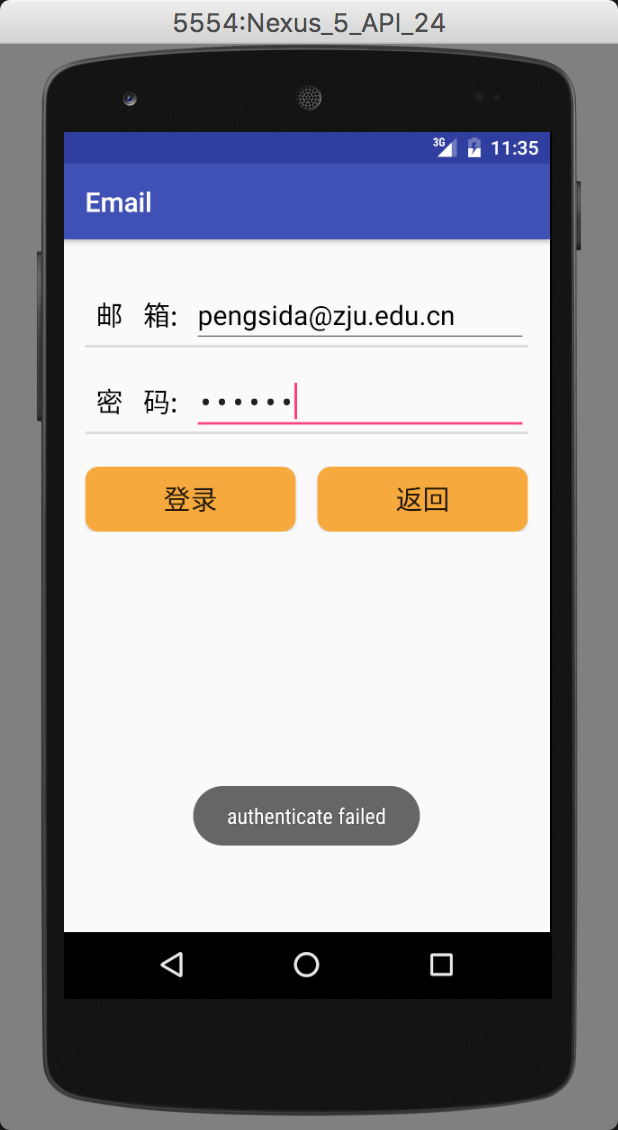
\includegraphics[width=0.3\textwidth]{2.png} &
	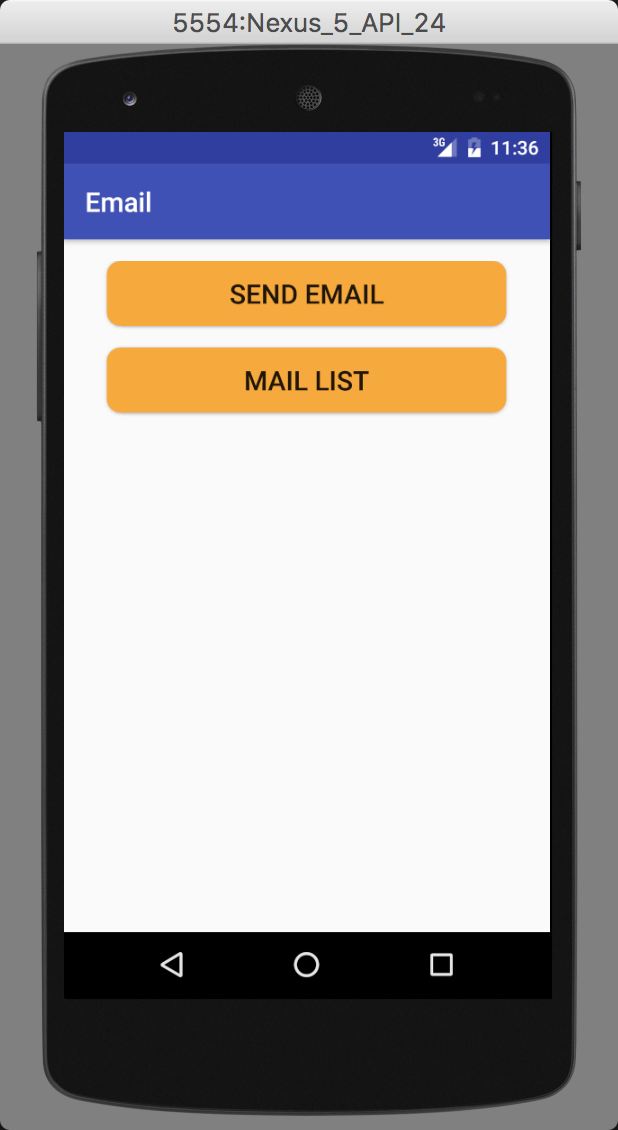
\includegraphics[width=0.3\textwidth]{3.png} \\
	\end{longtable}

\subsection{发邮件}
	在上述视图中,点击“SEND EMAIL”的按钮,就可以进入发邮件的视图,如下图所示:
	\sizedfic{0.3}{4.png}

	比如发送一封文本邮件,发给“291277604@qq.com”,主题为“Hello world”,内容为“From pengsida@zju.edu.cn”,
	随后我的QQ邮箱就收到了这封邮件,如下图所示:
	\begin{longtable}{p{0.3\textwidth}p{0.7\textwidth}}
	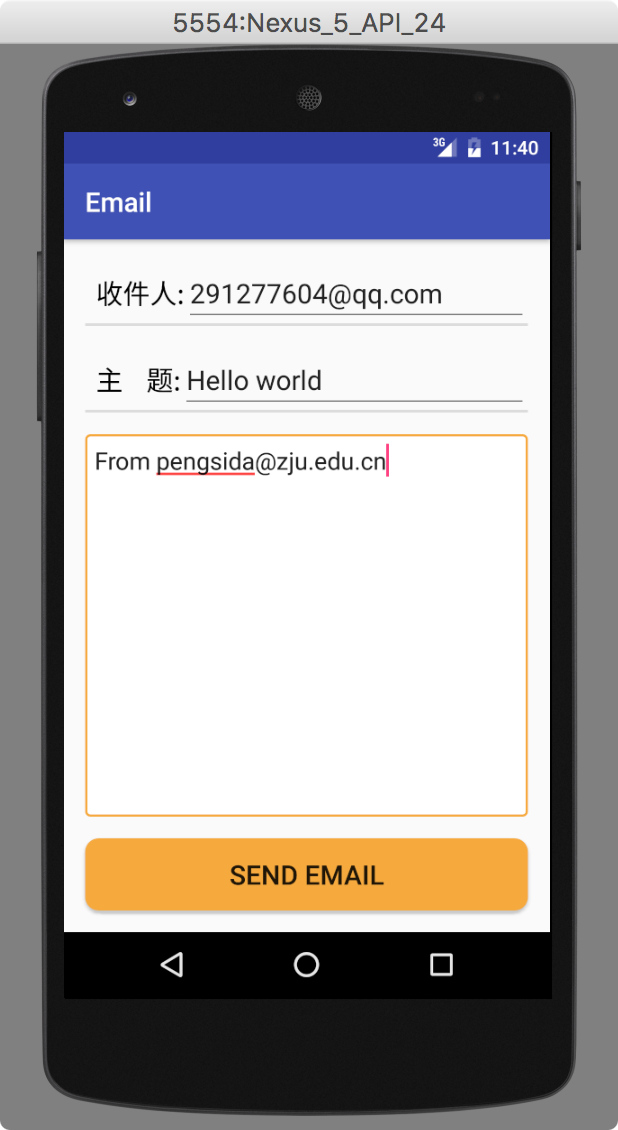
\includegraphics[width=0.3\textwidth]{5.png} &
	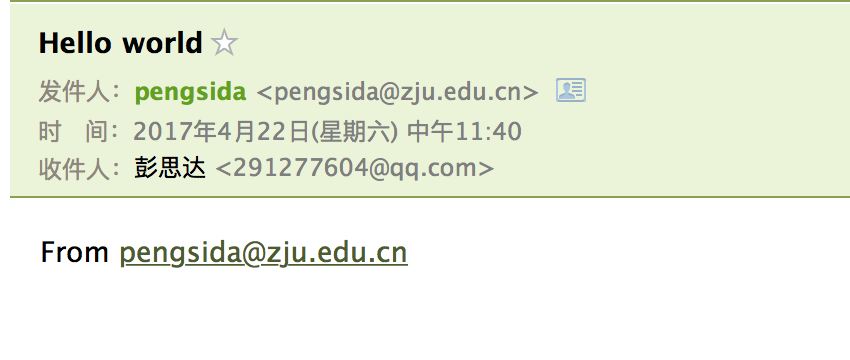
\includegraphics[width=0.7\textwidth]{6.png} \\
	\end{longtable}

\subsection{收邮件}
	在主界面中,点击“MAIL LIST”的按钮,就可以查看邮件列表,如下图所示:
	\sizedfic{0.3}{7.PNG}

	我的邮件客户端可以查看文本格式的邮件和多图文格式的邮件,文本格式的邮件和多图文格式的邮件如下所示:
	\begin{longtable}{p{0.3\textwidth}p{0.3\textwidth}}
	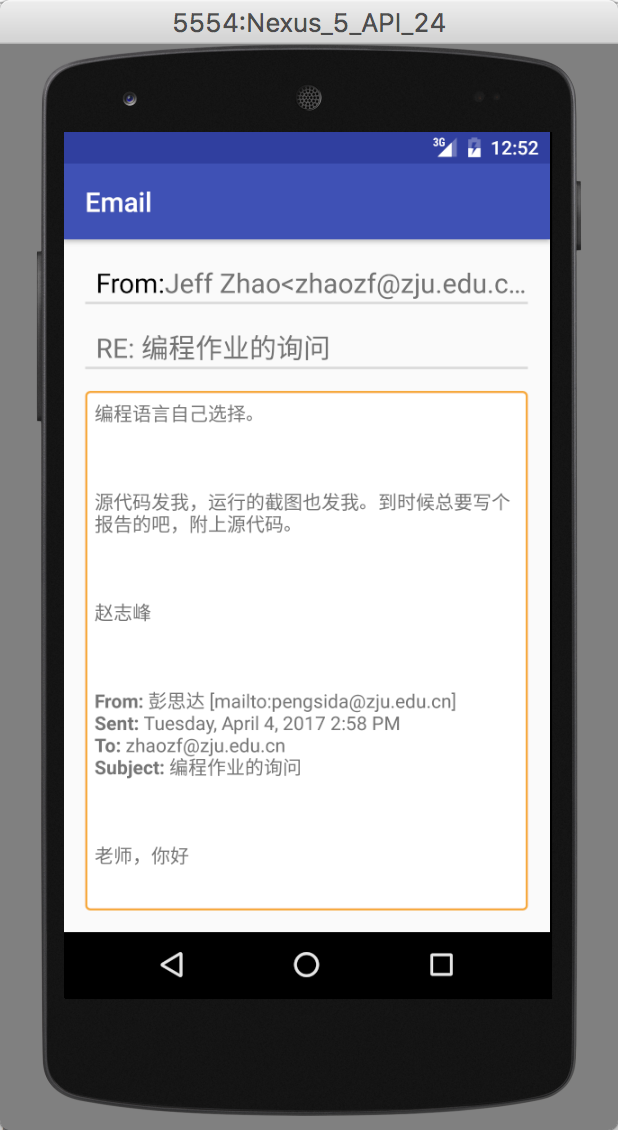
\includegraphics[width=0.3\textwidth]{8.png} &
	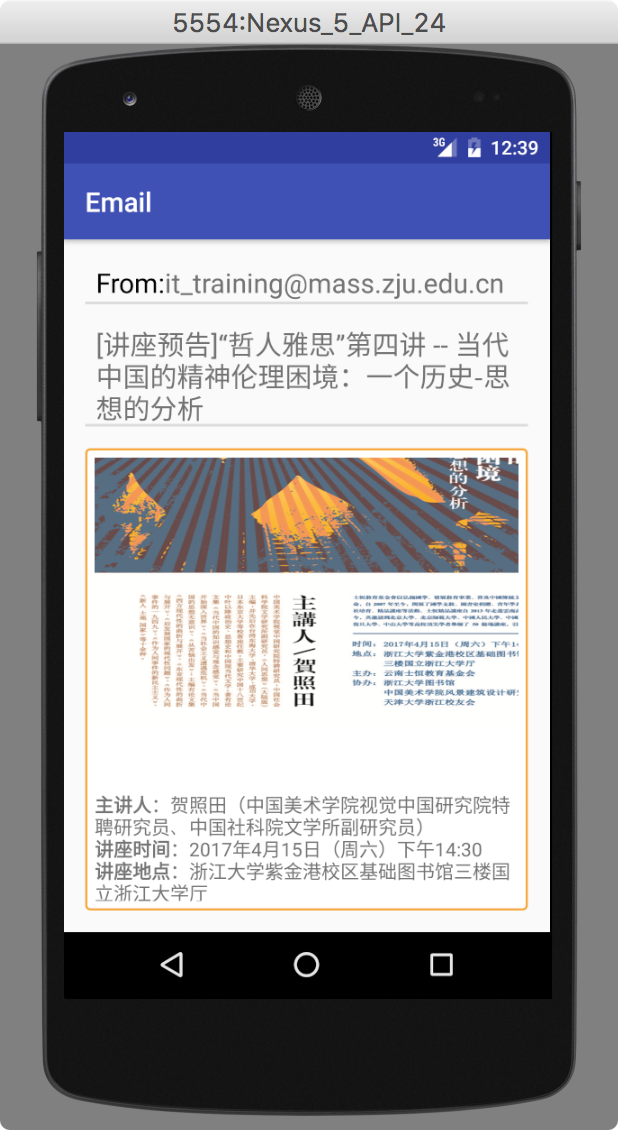
\includegraphics[width=0.3\textwidth]{9.png} \\
	\end{longtable}

\section{功能的实现}
	因为代码比较多,有两千多行,接下来我采取的策略是,讲述自己实现相应功能的方法并贴出关键的代码。
	整个文档看下来,只会了解大体的实现框架,如果想了解细节,需要去看附件中完整的代码。

\subsection{验证邮箱密码的实现}
	实现登陆邮箱的功能有如下步骤:
	\begin{itemize}
		\item[1.] 写一个登录界面。
		\item[2.] 通过JavaMail来进行邮箱密码的验证。
		\item[3.] 编写一个控制层,从而可以让用户可以交互使用,其中关键的组件是两个输入框和一个按钮。
	\end{itemize}

\clearpage

\subsubsection{首先画一个登录界面}
	android画一个界面还是比较简单的,只要编辑相应的代码,就能得到相应的界面。源码和相应的效果图如下所示,
	因为考虑到源码较多,这里只截取了一部分,如果想看完整的代码,可以查看附件:
	\fic{10.png}

\subsubsection{进行邮箱密码的验证}
	对于这一功能,我的基本想法是通过邮箱和密码连接smtp服务器,如果连接成功,就说明密码正确并登入主界面,如果不能连接成功,就说明密码错误并提示错误信息。\par

	我使用了JavaMail中的Session类、Transport类来验证邮箱。\par
	Session类是JavaMail API的主要类,它不创建子类。 Session 对象充当连接工厂的JavaMail API,它可以同时处理配置设置和身份验证。
	创建Session对象的一种方法是基于编程方法,可以在其中使用的java.util.Properties对象来覆盖一些默认信息,如邮件服务器名,用户名,密码,那可以是其他信息整个应用程序共享。
	如:Session session = Session.getDefaultInstance(new Properties());\par
	
	Transport类用来作为消息传输机制。这个类通常使用SMTP协议来发送消息。你可以通过只调用静态的send()方法使用该类的默认版本:Transport.send(message);\par

	实现这项功能的关键代码如下:

	\begin{lstlisting}
	Session session = Session.getDefaultInstance(new Properties());

    try
    {
        Transport transport = session.getTransport("smtp");
        String mailboxKey = resolve(mailbox);
		
		// smtpServerList是我的邮件客户端可以支持的邮件服务器
		// 目前可以支持qq邮箱和浙大邮箱
		// 要支持一个邮箱,只需要在smtpServerList中添加相应的smtp服务器即可
        transport.connect(smtpServerList.get(mailboxKey), Integer.parseInt(portList.get(mailboxKey)), mailbox, passwd);
        return "right";
    }
    catch (AuthenticationFailedException ea)
    {
        return "authenticate failed";
    }
    catch (MessagingException em)
    {
        return "wrong";
    }
	\end{lstlisting}

\subsubsection{编写一个控制层}
	这里定义了视图层的三个组件:邮箱文本框、密码文本框和登录按钮。
	邮箱文本框用于输入邮箱账号,密码文本框用于输入密码,登陆按钮用于测试密码是否正确。\par

	实现邮箱文本框和密码文本框的关键代码如下:
	\begin{lstlisting}
	mailboxEditText.addTextChangedListener(new TextWatcher() {
		...

		@Override
		public void onTextChanged(CharSequence s, int start, int before, int count)
		{
			mailbox = s.toString();
		}

		...
	});

	passwdEditText.addTextChangedListener(new TextWatcher() {
		...

		@Override
		public void onTextChanged(CharSequence s, int start, int before, int count)
		{
			passwd = s.toString();
		}

		...
	});
	\end{lstlisting}

	实现登录按钮的关键代码如下:
	\begin{lstlisting}
	loginButton.setOnClickListener(new View.OnClickListener() {
		@Override
		public void onClick(View v)
		{
			...
			new VerifyPasswd().execute();
		}
	});
	\end{lstlisting}

	上面的VerifyPasswd类是一个异步线程类,因为android不允许主线程使用网络,所以只能另开一个异步线程,如下所示:
	\begin{lstlisting}
	private class VerifyPasswd extends AsyncTask<Void, Void, String>
    {
        @Override
        protected String doInBackground(Void... params)
        {
            Session session = Session.getDefaultInstance(new Properties());

            try
            {
                Transport transport = session.getTransport("smtp");
                String mailboxKey = resolve(mailbox);
                transport.connect(smtpServerList.get(mailboxKey), Integer.parseInt(portList.get(mailboxKey)), mailbox, passwd);
                return "right";
            }
            catch (AuthenticationFailedException ea)
            {
                return "authenticate failed";
            }
            catch (MessagingException em)
            {
                return "wrong";
            }
        }

        @Override
        protected void onPostExecute(String text)
        {
            if (text.equals("right"))
            {
                Map<String, String> keys = new HashMap<String, String>();
                putIntentData(keys);
                Intent i = MainActivity.newIntent(LoginActivity.this, keys);
                startActivity(i);
            }
            else
                Toast.makeText(LoginActivity.this, text, Toast.LENGTH_SHORT).show();
        }
    }
	\end{lstlisting}

\clearpage

\subsection{发邮件的实现}
	实现发邮件的功能有如下步骤:
	\begin{itemize}
		\item[1.] 写一个发邮件的界面。
		\item[2.] 通过JavaMail来进行邮件的发送。
		\item[3.] 编写一个控制层,从而可以让用户可以交互使用,其中关键的组件是三个输入框和一个按钮。
	\end{itemize}

\subsubsection{发邮件界面的实现}
	部分代码和界面如下图所示:
	\fic{11.png}

\subsubsection{通过JavaMail来实现发送邮件的功能}
	我使用了JavaMail中的Session类、Authenticator类、Message类、Address类和Transport类来实现发送邮件的功能。\par

	Authenticator类表示懂得如何获得认证的网络连接的对象。它是一个抽象类。您可以创建一个子类PasswordAuthentication,通过用户名和密码给它的构造。
	代码实现如下:
	\begin{lstlisting}
	public class MyAuthenticator extends Authenticator
	{
		private String userName;
		private String password;

		public MyAuthenticator(String userName, String password)
		{
			this.userName = userName;
			this.password = password;
		}

		@Override
		protected PasswordAuthentication getPasswordAuthentication()
		{
			// 创建一个子类PasswordAuthentication,通过用户名和密码给它的构造
			return new PasswordAuthentication(userName, password);
		}

		...
	}
	\end{lstlisting}

	我们通过Authenticator类来构造一个Session对象:
	\begin{lstlisting}
	// MailSenderInfo是我自定义的一个类
	// 它用于存放发送邮箱所需要的信息
	public static boolean sendTextMail(MailSenderInfo mailInfo)
    {
        MyAuthenticator authenticator = null;
        if(mailInfo.isValidate())
            authenticator = new MyAuthenticator(mailInfo.getUserName(), mailInfo.getPassword());

        Session sendMailSession = Session.getInstance(mailInfo.getProperties(), authenticator);
		...
	}
	\end{lstlisting}

	Address类是一个抽象类。因此,它的子类javax.mail.internet.InternetAddress类大多被使用,它用于表示邮件发送中的地址对象。
	Address可以通过电子邮件地址来创建:
	\begin{lstlisting}
	// 创建收件箱和发件箱的地址对象
	Address from = new InternetAddress(mailInfo.getFromAddress());
	Address to = new InternetAddress(mailInfo.getToAddress());
	\end{lstlisting}

	Message类是一个抽象类。因此,它的子类javax.mail.internet.MimeMessage类大多使用,它用于表示邮件这个对象。
	我们要对其设置发件人、收件人、邮件主题、发件日期、邮件内容,代码如下:
	\begin{lstlisting}
	Message mailMessage = new MimeMessage(sendMailSession);
	Address from = new InternetAddress(mailInfo.getFromAddress());
	// 设置发件人
	mailMessage.setFrom(from);
	Address to = new InternetAddress(mailInfo.getToAddress());
	// 设置收件人
	mailMessage.setRecipient(Message.RecipientType.TO, to);
	// 设置邮件主题
	mailMessage.setSubject(mailInfo.getSubject());
	// 设置发件日期
	mailMessage.setSentDate(new Date());
	String mailContent = mailInfo.getContent();
	// 设置邮件内容
	mailMessage.setText(mailContent);
	\end{lstlisting}

	最后使用Transport类发送邮件:
	\begin{lstlisting}
	Transport.send(mailMessage);
	\end{lstlisting}

	完整代码如下:
	\begin{lstlisting}
	public static boolean sendTextMail(MailSenderInfo mailInfo)
    {
        MyAuthenticator authenticator = null;
        if(mailInfo.isValidate())
            authenticator = new MyAuthenticator(mailInfo.getUserName(), mailInfo.getPassword());

        Session sendMailSession = Session.getInstance(mailInfo.getProperties(), authenticator);

        try {
            Message mailMessage = new MimeMessage(sendMailSession);
            Address from = new InternetAddress(mailInfo.getFromAddress());
            mailMessage.setFrom(from);
            Address to = new InternetAddress(mailInfo.getToAddress());
            mailMessage.setRecipient(Message.RecipientType.TO, to);
            mailMessage.setSubject(mailInfo.getSubject());
            mailMessage.setSentDate(new Date());
            String mailContent = mailInfo.getContent();
            mailMessage.setText(mailContent);

            Transport.send(mailMessage);
            return true;
        }
        catch (MessagingException ex)
        {
            ex.printStackTrace();
        }

        return false;
    }
	\end{lstlisting}

\subsubsection{编写一个控制层}
	这里定义了视图层的四个组件:收件人文本框、主题文本框、内容文本框和发件按钮。\par

	实现收件人文本框、主题文本框和内容文本框的关键代码如下:
	\begin{lstlisting}
	toAddressEditText.addTextChangedListener(new TextWatcher() {
		...
		@Override
		public void onTextChanged(CharSequence s, int start, int before, int count)
		{
			toAddress = s.toString();
		}
		...
	});

	subjectEditText.addTextChangedListener(new TextWatcher() {
		...
		@Override
		public void onTextChanged(CharSequence s, int start, int before, int count)
		{
			subject = s.toString();
		}
		...
	});

	contentEditText.addTextChangedListener(new TextWatcher() {
		...
		@Override
		public void onTextChanged(CharSequence s, int start, int before, int count)
		{
			content = s.toString();
		}
		...
	});
	\end{lstlisting}

	发件按钮的实现如下:
	\begin{lstlisting}
	sendEmailButton.setOnClickListener(new View.OnClickListener() {
		@Override
		public void onClick(View v)
		{
			new Thread(sendEmail).start();
			finish();
		}
	});
	\end{lstlisting}

	其中sendEmail是一个用于发送邮件的线程:
	\begin{lstlisting}
	Runnable sendEmail = new Runnable() {
        @Override
        public void run() {
            Looper.prepare();
            MailSenderInfo mailSenderInfo = new MailSenderInfo();
            mailSenderInfo.setMailServerHost(smtpServer);
            mailSenderInfo.setMailServerPort("25");
            mailSenderInfo.setValidate(true);
            mailSenderInfo.setUserName(mailbox);
            mailSenderInfo.setPassword(passwd);
            mailSenderInfo.setFromAddress(mailbox);
            mailSenderInfo.setToAddress(toAddress);
            mailSenderInfo.setSubject(subject);
            mailSenderInfo.setContent(content);
            MailSender.sendTextMail(mailSenderInfo);
        }
    };
	\end{lstlisting}

\subsection{收邮件的实现}
	实现收邮件的功能有如下步骤:
	\begin{itemize}
		\item[1.] 写一个邮件列表的界面和一个邮件明细界面。
		\item[2.] 通过JavaMail来进行邮件的接收。
		\item[3.] 编写一个控制层,让用户可以看到邮件列表和查看特定的邮件。
	\end{itemize}

\subsubsection{写一个邮件列表的界面和一个邮件明细界面}
	邮件列表的界面是用RecyclerView实现的,这是一个比较高级的组件,有兴趣的读者可以深入去了解一下。
	它的功能实现会在控制层交代,这里只是画一个界面:
	\fic{12.png}

	邮件明细界面就相对简单一些,如下所示:
	\fic{13.png}

\subsubsection{通过JavaMail来进行邮件的接收}
	我使用了JavaMail中的Folder类、Store类、Message类。
	这里的Folder类和Store类主要用于打开收件箱,
	为了完成邮件的接收和显示,我们还需要解析Message对象,这是这一部分的难点。\par

	Store类是一个抽象类,模型信息存储和访问协议,用于存储和检索信息。
	子类提供实际的实现。存储扩展服务类,它提供命名商店,连接到存储,并听取连接事件很多常见的方法。
	客户获得通过获得它实现了数据库访问协议的Store对象访问消息存储。大多数邮件存储需要进行身份验证,才允许访问的用户。 
	connect方法进行身份验证。\par

	代码中对Store对象的获取如下所示:
	\begin{lstlisting}
	public void connectToServer() throws MessagingException
    {
        MyAuthenticator authenticator = null;
        if(this.receiverInfo.isValidate())
            authenticator = new MyAuthenticator(this.receiverInfo.getUserName(), this.receiverInfo.getPassword());

        Session session = Session.getInstance(this.receiverInfo.getProperties(), authenticator);

        try
        {
			// 获得Store对象
            this.store = session.getStore(this.receiverInfo.getProtocal());
        }
        catch (NoSuchProviderException e)
        {
            e.printStackTrace();
            throw new MessagingException("连接服务器失败!");
        }

        System.out.println("connecting");

        try
        {
			// 连接到服务器
            this.store.connect();
        }
        catch (MessagingException e)
        {
            throw new MessagingException("连接服务器失败!");
        }

        System.out.println("连接服务器成功");
    }
	\end{lstlisting}

	Folder类是表示一个文件夹的邮件消息的抽象类。子类实现协议的具体文件夹。文件夹可以包含子文件夹,以及消息,从而提供了一种分层结构。
	连接到存储后,您就可以得到一个文件夹,必须先打开,然后才能从中读取消息。
	我们在代码中打开收件箱的操作如下:
	\begin{lstlisting}
	public void openInBoxFolder() throws MessagingException
    {
        try {
            this.folder = this.store.getFolder("INBOX");
            folder.open(Folder.READ_ONLY);
        }
        catch (MessagingException e)
        {
            throw new MessagingException("打开收件箱失败!");
        }
    }
	\end{lstlisting}

	接下来就是获取Message对象并解析Message对象。获取Message对象如下所示:
	\begin{lstlisting}
	Message[] messages = this.folder.getMessages();
	\end{lstlisting}

	但是,这里获得的messages都是乱序的,不是按照日期排序的,我们还需要对其进行排序。
	这里使用了Java中的Collections类进行排序:
	\begin{lstlisting}
	// 获得邮件对象
	messages = myMessage.getMessages();
	
	// 这里的MailItem是我定义的一个类,用于存放邮件的一些信息
	// 稍后在控制层中可以看到,mailItemList会和recyclerview配合使用
	ArrayList<MailItem> mailItemList = new ArrayList<MailItem>();

	for (int index = 0; index < messages.length; ++index)
	{
		try {
			MessageResolver messageResolver = new MessageResolver(messages[index]);
			mailItemList.add(new MailItem(messages[index], messageResolver.getSubject(), messageResolver.getSentDate()));
		}
		catch (MessagingException e)
		{
			e.printStackTrace();
		}
	}
	// MailItem是Comparable的一个子类,所以可以用Collections排序
	// 具体实现见附件中的代码
	Collections.sort(mailItemList);
	\end{lstlisting}

	解析Message对象的算法如下:
	\begin{itemize}
		\item[1.] 首先判断Message对象是不是一个附件,如果是,就直接保存它的内容。
		\item[2.] 随后判断Message对象的类型。
		\item[3.] 如果Message对象是具体一个文件类型的邮件,就直接得到它的内容。
		\item[4.] 如果Message对象的类型是multipart,就循环得到它的各个part,然后再递归解析各个part对象。
	\end{itemize}

	实现解析功能的代码如下:
	\begin{lstlisting}
	private void saveEveryPartOfMessage(String dirName, Part part) throws IOException, MessagingException
    {
        String disposition = part.getDisposition();
        String contentType = part.getContentType();

		// 判断Message对象是不是一个附件
        if (disposition != null)
        {
            String filename = getFileName(dirName, part);
            System.out.println("邮件附件的存储路径:" + filename);
            saveFile(part, filename);
            return;
        }

		// 判断Message对象的类型
        if (contentType.contains("multipart"))
        {
            DataSource source = new ByteArrayDataSource(part.getInputStream(), "multipart/*");
            Multipart mp = new MimeMultipart(source);

            for (int index = 0; index < mp.getCount(); ++index)
                saveEveryPartOfMessage(dirName, mp.getBodyPart(index));
        }
        else
        {
            if (contentType.contains("text/plain"))
            {
                String filename = getFileName(dirName, part);
                System.out.println("邮件txt文件的存储路径:" + filename);
                saveFile(part, filename);
            }
            else if(contentType.contains("text/html"))
            {
                String filename = getFileName(dirName, part);
                System.out.println("邮件html文件的存储路径:" + filename);
                saveFile(part, filename);
            }
        }
    }
	\end{lstlisting}

	收邮件的功能其实到这里就结束了,我们可以得到邮件的各个部分。
	但是需要知道的是,我们是想实现一个android应用,不可能只是把邮件的各部分简单地保存到本地,我们还需要把它的内容显示出来,这在控制层会讲如何实现。

\clearpage

\subsubsection{编写一个控制层}
	控制层主要想实现的功能是,能显示邮件列表,然后能显示邮件内容。邮件列表是recyclerview实现的,邮件内容的显示是通过三个textview实现的。
	其中两个textview是显示发件人和邮件主题,最后一个textview用于显示邮件内容。

\subsubsection{recyclerView的实现}

	首先来说recyclerview,我们为了实现它,需要写一个MailItemHolder类和一个MailItemAdapter类。
	简单来说,MailItemHolder类用于显示每个MailItem,MailItemAdapter类用于将MailItemHolder类和特定的MailItem绑定起来。
	\begin{lstlisting}
	private class MailItemHolder extends RecyclerView.ViewHolder implements View.OnClickListener
    {
        public TextView subjectTextView;
        public TextView dateTextView;
        public Message message;

        public MailItemHolder(View itemView)
        {
            super(itemView);
            itemView.setOnClickListener(this);
            subjectTextView = (TextView)itemView.findViewById(R.id.from_and_subject_info);
            dateTextView = (TextView)itemView.findViewById(R.id.date_info);
        }

        @Override
        public void onClick(View v)
        {
            myMessage.setMessage(this.message);
            Intent i = MailDetailActivity.newIntent(MailListActivity.this);
            startActivity(i);
        }
    }

    private class MailItemAdapter extends RecyclerView.Adapter<MailItemHolder>
    {
        private List<MailItem> mailItemList;
        private DateFormat dateFormat = new SimpleDateFormat("yyyy-MM-dd HH:mm:ss");

        public MailItemAdapter(List<MailItem> mailItemList)
        {
            this.mailItemList = mailItemList;
        }

        @Override
        public MailItemHolder onCreateViewHolder(ViewGroup parent, int viewType)
        {
            LayoutInflater layoutInflater = LayoutInflater.from(MailListActivity.this);
            View view = layoutInflater.inflate(R.layout.received_mail_item, parent, false);
            return new MailItemHolder(view);
        }

        @Override
        public void onBindViewHolder(MailItemHolder holder, int position)
        {
            if (mailItemList == null)
                return;
            holder.subjectTextView.setText(mailItemList.get(position).getSubject());
            holder.dateTextView.setText(dateFormat.format(mailItemList.get(position).getDate()));
            holder.message = mailItemList.get(position).getMessage();
        }

        @Override
        public int getItemCount()
        {
            if (mailItemList == null)
                return 0;
            return this.mailItemList.size();
        }
    }
	\end{lstlisting}

	实现这两个类以后,只要在通过如下两行代码,就能让recyclerview显示邮件列表:
	\begin{lstlisting}
	mailItemAdapter = new MailItemAdapter(mailItemList);
	recyclerView.setAdapter(mailItemAdapter);
	\end{lstlisting}

\subsubsection{显示邮件内容}
	前两个textview分别用于显示显示发件人和邮件主题,代码如下:
	\begin{lstlisting}
	private class GetMessages extends AsyncTask<Void, Void, Void>
    {
        @Override
        protected Void doInBackground(Void... params)
        {

            try
            {
                myMessage.openInBoxFolder();
				
				// MessageResolver是我定义的一个类,用于解析Message对象
                messageResolver = new MessageResolver(myMessage.getMessage());
                fromAddress = messageResolver.getFrom();
                subject = messageResolver.getSubject();
                ...
            }
            catch (MessagingException e)
            {
                e.printStackTrace();
            }
            catch (IOException e)
            {
                e.printStackTrace();
            }
            return null;
        }

        @Override
        protected void onPostExecute(Void params)
        {
			// 显示发件人和邮件主题
            fromAddressTextView.setText(fromAddress);
            subjectTextView.setText(subject);
			...
        }
    }
	\end{lstlisting}

	最后一个textview用于显示邮件内容,算法如下:
	\begin{itemize}
		\item[1.] 获得邮件的类型。
		\item[2.] 如果邮件是“text/plain”类型的,就直接显示邮件内容。
		\item[3.] 如果邮件是“text/html”类型的,就将邮件内容转码以后显示。
		\item[4.] 如果邮件是“multipart/related”类型的,说明邮件是多图文的,需要将附件中的图片存入本地,然后将html文本中img标签的src路径改为本地路径,从而在textview显示出来。
		\item[5.] 如果邮件是其它类型的,就分别得到其中的“HTML”内容,如果该内容为空,就得到其中的“PLAIN”内容。
	\end{itemize}

	实现代码如下:
	\begin{lstlisting}
	private class GetMessages extends AsyncTask<Void, Void, Void>
    {
        @Override
        protected Void doInBackground(Void... params)
        {
            try
            {
                myMessage.openInBoxFolder();
                messageResolver = new MessageResolver(myMessage.getMessage());
                ...
                contentType = messageResolver.getContentType();
                if (contentType.contains("text/plain") || contentType.contains("text/html"))
                    content = myMessage.getMessage().getContent().toString();
                else if (contentType.contains("multipart/related"))
                {
                    File externalFilesDir = MailDetailActivity.this.getExternalFilesDir(Environment.DIRECTORY_PICTURES);
                    if(externalFilesDir == null)
                    {
                        Toast.makeText(MailDetailActivity.this, "Wrong", Toast.LENGTH_SHORT).show();
                        return null;
                    }
                    Log.d("OPEN", externalFilesDir.toString());
                    dirName = externalFilesDir.toString();

                    content = messageResolver.getHtmlContent(dirName);
                    if (content.contains("<style>"))
                    {
                        int start = content.indexOf("<style>");
                        int end = content.indexOf("</style>");
                        content = content.substring(0, start) + content.substring(end+8);
                    }

                    text_or_html = false;
                }
                else if (contentType.contains("multipart"))
                {
                    content = messageResolver.getHtmlContent("NULL");
                    if (content == null || content.equals(""))
                    {
                        content = messageResolver.getPlainContent();
                        text_or_html = true;
                    }
                    else
                    {
                        if (content.contains("<style>"))
                        {
                            int start = content.indexOf("<style>");
                            int end = content.indexOf("</style>");
                            content = content.substring(0, start) + content.substring(end+8);
                        }
                        text_or_html = false;
                    }
                }
                else
                    content = "";
            }
            catch (MessagingException e)
            {
                e.printStackTrace();
            }
            catch (IOException e)
            {
                e.printStackTrace();
            }
            return null;
        }

        @Override
        protected void onPostExecute(Void params)
        {
            ...
            String temp = "<img src=\"/storage/emulated/0/Android/data/psd.email/files/Pictures/test.jpg\" />";
            if (contentType.contains("multipart") && content != null)
            {
                if (contentType.contains("multipart/related"))
                {
                    content = FormatHtml.stringFormat(content);
                    contentView.setText(Html.fromHtml(content, imageGetter, null));
                }
                else
                {
                    if (text_or_html)
                        contentView.setText(content);
                    else
                        contentView.setText(Html.fromHtml(content));
                }
            }
            else if (contentType.contains("text/plain"))
                contentView.setText(Html.fromHtml(content));
            else
                contentView.setText(content);
        }
    }
	\end{lstlisting}

	其中FormatHtml.stringFormat()函数是我用来处理html文本的,代码如下:
	\begin{lstlisting}
	public class FormatHtml
	{
		public static String stringFormat(String html)
		{
			Pattern pattern = Pattern.compile("<img src=\"cid.*?>");
			Matcher matcher = pattern.matcher(html);
			System.out.println(matcher.replaceFirst("<img src=\"/storage/emulated/0/Android/data/psd.email/files/Pictures/test.jpg\" />"));
			String s = matcher.replaceFirst("<img src=\"/storage/emulated/0/Android/data/psd.email/files/Pictures/test.jpg\" />");
			pattern = Pattern.compile("<img src=\"http.*?>");
			matcher = pattern.matcher(s);
			return matcher.replaceFirst("");
		}
		...
	}
	\end{lstlisting}

\end{document}
